%============================================================
% titlepage.tex
%============================================================
\begin{titlepage}
\begin{tikzpicture}[remember picture, overlay]
    \fill[primaryblue] ([yshift=-2.2cm]current page.north west) rectangle ([yshift=-2.35cm]current page.north east);
    \fill[accentorange] ([yshift=-2.5cm]current page.north west) rectangle ([yshift=-2.56cm]current page.north east);
    \fill[primaryblue] ([yshift=2.2cm]current page.south west) rectangle ([yshift=2.35cm]current page.south east);
\end{tikzpicture}
\centering
\vspace*{2.5cm}

{\fontsize{44}{52}\selectfont\bfseries\color{primaryblue} Arrays\par}
\vspace{0.4cm}
{\LARGE\bfseries\color{deepblue} From Foundations to World Finals\par}
\vspace{0.8cm}

% emblem: an array with a sliding window, two pointers and its prefix sums
\begin{tikzpicture}[scale=1.0]
    \dparray{a}{0}{$a$}{3/aout, 1/awin, 4/awin, 1/awin, 5/awin, 9/acell, 2/acell, 6/acell}
    \dparray{p}{-1.6}{$P$}{3/compcell, 4/compcell, 8/compcell, 9/compcell, 14/anscell, 23/compcell, 25/compcell, 31/compcell}
    \aptrup{a1}{l}{successgreen}
    \aptrup{a4}{r}{accentorange}
    \arange{a1}{a4}{sum = 11 = 14 $-$ 3}{memoorange}
\end{tikzpicture}
\par\vspace{0.3cm}
{\small\itshape\color{darkgray} an index, a range, a loop --- and the right invariant\par}
\vspace{1.2cm}

\begin{tcolorbox}[enhanced, colback=white, colframe=primaryblue, boxrule=1.5pt,
                  arc=3mm, width=0.78\textwidth, halign=center]
\textcolor{primaryblue}{\textbf{6 Parts}}
\textcolor{darkgray}{$\bullet$}
\textcolor{primaryblue}{\textbf{36 Chapters}}
\textcolor{darkgray}{$\bullet$}
\textcolor{accentorange}{\textbf{1000+ Problems}}
\textcolor{darkgray}{$\bullet$}
\textcolor{successgreen}{\textbf{Beginner $\to$ CF 3500}}
\end{tcolorbox}

\vfill
{\Large\color{darkgray} Himanshu Kumar\par}
\vspace{0.2cm}
{\color{darkgray}\today\par}
\vspace{1.5cm}
\end{titlepage}
